\documentclass[pdflatex,sn-basic,Numbered]{sn-jnl}
\usepackage{graphicx}
\usepackage{multirow}
\usepackage{amsmath,amssymb,amsfonts}
\usepackage[title]{appendix}
\usepackage{xcolor}
\usepackage{booktabs}
\usepackage{manyfoot}
\usepackage{tikz}
\usetikzlibrary{shapes.geometric, arrows.meta, positioning}
\raggedbottom

\begin{document}

\title{Whose Art Counts? Model- and Prompt-Dependent Associations in Vision-Language Judgments of Museum Art}

\author*[1]{\fnm{Manpreet} \sur{Singh}}\email{manni@bu.edu}
\author[2]{\fnm{Nandakishor Reddy} \sur{Pulagam}}\email{pulagamnkr@gmail.com}
\author[3]{\fnm{Rhythm} \sur{Bhatia}}\email{bhatiarhythm06@gmail.com}
\author*[4]{\fnm{Rahul} \sur{Joshi}}\email{rahulj@sitpune.edu.in}

\affil*[1]{\orgname{Boston University}, \orgaddress{\city{Boston}, \state{MA}, \country{USA}}}
\affil[2]{\orgname{Independent Researcher}}
\affil[3]{\orgname{University of Eastern Finland}, \orgaddress{\country{Finland}}}
\affil[4]{\orgname{Symbiosis Institute of Technology, Symbiosis International University}, \orgaddress{\city{Pune}, \country{India}}}

\abstract{
Vision-language models are increasingly used to search, rank, and describe cultural collections. Their judgments of artistic value may reflect both learned image-text associations and the structure of the archives on which those judgments are applied. We introduce an archive-conditioned audit design that treats model, prompt, and metadata provenance as parts of one measurement procedure. We test the design on 445 publicly accessible museum object images from the Metropolitan Museum of Art Open Access collection using four vision-language models: OpenAI CLIP, OpenCLIP ViT-B/32, OpenCLIP ViT-L/14, and SigLIP. The comparison cohort contains 61 works divided into two metadata-inferred creator categories, with 384 works remaining unknown or unattributed. We measure prompt-relative contrasts for masterpiece, quality, influence, and a generic-reference control. Influence prompts produce the clearest between-category differences for OpenAI CLIP and OpenCLIP L/14, while other prompts and models are inconsistent. An aggregate index is reported only as a secondary descriptive summary because prompt correlations are weak or mixed. Model scores use different scales, so cross-model diagnostics are computed only after within-model standardization. The primary contribution is an archive-conditioned measurement protocol. The Metropolitan Museum analysis demonstrates how the protocol can be applied in one query-defined archival setting. The findings do not establish artistic value, creator attributes, causal effects, or general model behavior. The project repository contains object-level manifests, prompts, score tables, and analysis code to support reproduction.
}

\keywords{Vision-language models, museum archives, digital humanities, prompt sensitivity, cultural-heritage AI, measurement protocols}

\maketitle

\section{Introduction}
\label{sec:introduction}

Vision-language models (VLMs) are now used for image retrieval, zero-shot classification, and collection analysis. CLIP established a widely used approach for connecting images and natural-language labels through contrastive pretraining on large image-text datasets \cite{radford2021learning}. Later systems, including OpenCLIP and SigLIP, use related image-text objectives with different training data, model sizes, and scoring conventions \cite{cherti2023reproducible, schuhmann2022laion}. These models can place an artwork near words such as ``masterpiece,'' ``quality,'' or ``influential.'' Such outputs are not direct observations of artistic merit. They are responses to a particular image, model, and phrase.

That distinction matters in cultural heritage applications. Machine-learning systems are already used for classification, retrieval, and analysis of cultural objects \cite{fiorucci2020machine, srinivasan2021arts}. A museum interface that ranks objects by a value-related prompt may therefore reproduce associations learned from web-scale data, from the visual properties of the image, or from the collection itself. Existing audits have found gender and racial disparities in visual-language systems, but most tests use benchmark images or broad demographic prompts \cite{wang2022revisiting, wolfe2022evidence, hall2023auditing}. Less attention has been paid to how these effects behave when the target is a historically situated cultural judgment.

Museum records are not neutral sampling frames. Acquisition, attribution, cataloging, and digitization determine which objects receive names, images, and descriptive fields. Studies of museum holdings have documented substantial imbalances in artist gender and geography \cite{topaz2019diversity, meier2021gender}. Classification systems also carry the institutional decisions through which objects become legible in an archive \cite{bowker2000sorting, noble2018algorithms, caswell2016archival}. A comparison of male- and female-attributed works after image filtering therefore describes a selected archival cohort. It cannot, by itself, distinguish a model association from differences in period, medium, department, image framing, or the survival of named records.

This study examines that measurement problem with publicly accessible museum object records from the Metropolitan Museum of Art Open Access collection. We ask whether creator-category differences in prompt-relative value scores are reproduced across four VLMs and four prompt contrasts within this query-defined audit cohort. The analysis treats model and prompt as a joint instrument. Agreement across instruments would strengthen an interpretation of a shared association. Disagreement would set a boundary on what can be claimed from any one model.

Our value-language prompts ask models to rank an image against a lower-valued alternative. Scores can reflect subject matter, composition, medium, photographic style, and learned associations, not artistic quality. They are probes of image-to-language mapping, distinct from recognition accuracy.

The archive creates a related interpretive boundary. A named artist is more likely to appear in the comparison than an anonymous workshop, an unidentified maker, or an object whose creator information was lost during cataloging. The 61-work comparison cohort is therefore not a census of artists represented by the museum. It is the portion of the image-complete corpus for which our conservative metadata procedure produced a binary analytic label. We retain the 384 unknown or unattributed works in the visual audit so that the model evaluation does not silently become an evaluation of named artists only.

Our research questions follow from these two boundaries:
\begin{enumerate}
    \item Are creator-category differences in prompt-relative value scores reproduced across model families?
    \item Which value prompts, if any, produce the most stable association?
    \item Do permutation and department-level sensitivity analyses change the interpretation of the aggregate comparison?
\end{enumerate}

The paper makes one primary contribution and three supporting contributions:
    \begin{enumerate}
    \item We define an archive-conditioned audit protocol that fixes the image cohort before inference, preserves unresolved records, and treats creator labels as metadata-derived analytic categories.
    \item We apply the protocol to the Metropolitan Museum collection, showing how three value-oriented prompts and a framing control behave across four VLMs on one fixed cohort.
    \item We instantiate the protocol with effect sizes, bootstrap intervals, within-model multiplicity correction, 10,000-label permutation tests, and department-composition sensitivity analysis.
    \item We specify a scale-aware comparison rule that keeps CLIP probabilities and SigLIP logits separate, then uses within-model standardization for cross-model instability analysis.
    \end{enumerate}

\section{Related work}
\label{sec:related}

This study draws on four related literatures: vision-language representation learning, multimodal fairness audits, machine learning for cultural heritage, and critical work on archival classification. They address different parts of the problem. VLM research explains how image-text scores are produced; fairness research supplies tests for group disparities; cultural-heritage research explains the application setting; and archival scholarship explains why the metadata cannot be treated as a neutral sampling frame.

\subsection{Vision-language representation learning}

CLIP learns a shared image-text representation from natural-language supervision and evaluates candidate labels through image-text similarity \cite{radford2021learning}. OpenCLIP extends this family with openly released training data and model variants, including models trained on LAION collections \cite{cherti2023reproducible, schuhmann2022laion}.
SigLIP uses a pairwise sigmoid loss instead of the batch-level softmax normalization employed by CLIP. As a result, the probability scores produced by CLIP and the logit scores generated by SigLIP are not directly comparable. Therefore, model performance is evaluated based on the direction of predictions, consistent prompting strategies, and standardized diagnostic measures, rather than on raw numerical values alone.

Softmax probabilities depend on the set of candidate labels included in the comparison, whereas SigLIP evaluates each image–text pair independently by assigning a logit score. Neither output should be interpreted as an absolute measure of image quality. A positive score simply indicates stronger support for the first text prompt relative to the second. For this reason, comparisons are restricted to results obtained from the same model using an identical set of prompts.

This approach is intended to support reliable measurement rather than conventional image classification. To ensure reproducibility, the complete prompts and model identifiers are reported so that future studies can examine alternative scoring methods or evaluation strategies rather than treating the reported scores as inherent properties of the artwork.

\subsection{Multimodal fairness and bias audits}

Previous studies have shown that multimodal datasets and vision-language models can encode associations related to gender, race, and sexuality \cite{birhane2021multimodal, wolfe2022evidence}. For example, Wang et al. examine gender and racial bias in CLIP using image-text evaluation tasks, while Hall et al. propose an auditing framework for assessing fairness and representation in vision-language models \cite{wang2022revisiting, hall2023auditing}. Their findings suggest that fairness cannot be judged from a single prediction or prompt. Rather, the evaluations should take into account multiple prompts and allow for uncertainty in the model's responses. The same kind of observation has been made in the wider fairness literature, where disparities are attributed not just to the model parameters but also to the composition of the dataset, the measurement decisions, and the deployment context \cite{buolamwini2018gender, mitchell2019model}. Drawing on this view, our study looks at cultural-value language by examining how the models react to terms like 'masterpiece' and 'influential' rather than focusing on traditional recognition accuracy.

Previous audit works distinguished between representational associations and actual real-world harms. The fact that different results were found in the controlled evaluation does not mean that the museum's recommendation system denied access, influenced curatorial decisions, or led to discriminatory outcomes; it only shows that the model's outputs depend on the image category or the way the prompt is worded. That is why we always refer to our findings as involving term associations rather than as evidence of downstream bias. This use of terminology does not assign a specific causal mechanism to the statistical differences and is consistent with recommendations regarding model cards and responsible reporting practices \cite{mitchell2019model}.

Even though balanced fairness benchmarks are useful for identifying how models behave, they usually fail to account for the circumstances in which the models are used. Museum collections are naturally uneven, as they reflect historical collecting practices and the cultural priorities of the time. Instead of eliminating this imbalance, our method preserves it, clearly records entries with unresolved metadata, and checks whether the observed associations differ across museum departments. By doing this, our approach supports benchmark-based audits by highlighting the significance of provenance and collection context.

\subsection{Machine learning for cultural heritage}

Machine learning has become a standard part of computational cultural-heritage research. Surveys describe applications in classification, retrieval, image analysis, and conservation, while digital humanities projects use computational representations to organize and interpret collections \cite{fiorucci2020machine, srinivasan2021arts}. These applications can increase access to collections, but they also make catalog structure consequential. A retrieval or ranking system can give greater visibility to objects that match the categories, visual conventions, or metadata fields favored by its model and prompt. The present study does not evaluate a deployed museum interface. It isolates one component of such a system: the prompt-relative score assigned to an image.

This component is worth isolating because ranking systems often turn continuous model scores into practical orderings. A small score difference may have little meaning in isolation but still affect which objects appear near the top of a search result. Conversely, a large difference that disappears under another model or prompt may be a property of the instrument rather than a stable property of the collection. By reporting model-specific scores, prompt-level effects, and standardized disagreement, our analysis makes that distinction explicit.

Cultural-heritage collections contain heterogeneous objects whose lighting, cropping, background, aspect ratio, and digitization quality may vary by medium and department. 
These factors complicate unconditioned comparisons. Our archive variables describe the context and support sensitivity analysis, but a clear limitation that they do not fully deconfound model responses.

\subsection{Archives, classification, and representation}

Archival classification is not a transparent mirror of the world. Bowker and Star describe classification systems as infrastructures that shape what can be recorded, compared, and retrieved \cite{bowker2000sorting}. Work on algorithmic oppression and archival silences makes a related point: categories can preserve institutional power while appearing administratively neutral \cite{noble2018algorithms, caswell2016archival}. Studies of museum holdings find persistent imbalances in artist gender and geography \cite{topaz2019diversity, meier2021gender}. These findings change how a museum VLM audit should be interpreted. Removing objects with unknown creators may make a statistical comparison easier, but it also removes part of the historical process under study. Our analysis reports this selection explicitly and treats the resolved binary comparison as conditional on archival survival and usable images.

The distinction between unknown and unattributed records is important. An unknown field may mean that the catalog does not provide enough information for our procedure. An unattributed object may have a collective, anonymous, workshop, or unresolved history. These cases should not be collapsed into evidence about a particular creator category. We use ``unknown or unattributed'' as an analytic boundary and preserve the underlying object records for future work that may use curatorial expertise, biographical databases, or non-binary attribution schemes.

Archival selection can also create a form of conditioning. Works with surviving names and usable images enter the comparison, while works whose makers were not recorded or whose images are unavailable do not. If those omissions correlate with medium, period, region, or gendered labor, the named comparison may not represent the collection that generated it. The leave-one-department-out analysis cannot solve this problem, but it can show whether the measured association is concentrated in one institutional segment within this query-defined cohort. We treat that evidence as a composition check, not as a correction for historical erasure.

\subsection{Position of the present study}

Table~\ref{tab:relatedwork} places this study beside selected works that are closest in method or application. The table is a focused comparison, not a systematic review of every VLM fairness or digital-heritage paper. The main difference is a measurement protocol that combines a museum archive, value-oriented prompt contrasts, multiple model families, and collection-composition sensitivity analysis.

The comparison is organized around unit of analysis. VLM papers study representations, fairness papers output disparities, cultural-heritage papers computational access, and archival scholarship classification. Our protocol connects these units through image scores, prompts, archive metadata, and selection paths.

The study provides a measurement protocol, not a new architecture, universal gender estimate, or museum-digitization survey.

\begin{table*}[htbp]
\centering
\caption{Selected related work and position of this study}
\label{tab:relatedwork}
\scriptsize
\resizebox{\textwidth}{!}{%
\begin{tabular}{p{0.18\textwidth}p{0.18\textwidth}p{0.19\textwidth}p{0.19\textwidth}p{0.18\textwidth}}
\toprule
Work & Main setting & Primary object of analysis & Main limitation for present question & Relation to this study \\
\midrule
Radford et al. \cite{radford2021learning} & General image-text pretraining & Zero-shot image-text representation & Not a fairness or cultural-heritage audit & Supplies CLIP foundation used by one model \\
Birhane et al. \cite{birhane2021multimodal} & Large multimodal datasets & Dataset stereotypes and harmful associations & Dataset-level analysis, not museum value judgments & Motivates checking inherited multimodal associations \\
Wang et al. \cite{wang2022revisiting} & CLIP fairness benchmarks & Gender and racial bias in image-text scores & Benchmark prompts and images, not archival selection & Provides closest fairness-audit precedent \\
Wolfe and Caliskan \cite{wolfe2022evidence} & Visual-language models & Gender-associated visual-language evidence & Broad demographic associations, not cultural value & Supports gender-sensitive prompt testing \\
Hall et al. \cite{hall2023auditing} & Visual-language model auditing & Fairness and representation evaluation & Does not center museum archives or artist attribution & Informs multi-model audit design \\
Fiorucci et al. \cite{fiorucci2020machine} & Cultural-heritage machine learning & Classification, retrieval, and image analysis & Survey rather than creator-category fairness test & Establishes application context \\
Topaz et al. \cite{topaz2019diversity} & Major U.S. museums & Artist gender and geographic representation & Collection representation, not VLM scoring & Motivates archival composition analysis \\
This study & Met museum artwork images & Prompt-relative artistic-value associations & One collection; small named comparison & Four VLMs, four prompts, permutation tests, and department sensitivity \\
\bottomrule
\end{tabular}%
}
\end{table*}

We do not propose a new VLM, fairness metric, or general estimate of gender bias in art. We propose and instantiate a protocol for applying familiar VLM scores to archives with uneven attribution and digitization histories. The museum case shows why model disagreement and archival selection must be reported together.

\section{Data and archival selection}
\label{sec:data}

\subsection{Source collection and unit of analysis}

We used records from the Metropolitan Museum of Art Open Access API \cite{met_api_2023}. The API record is the basic unit of analysis: one museum object, one selected image, and one set of catalog metadata. This keeps the statistical unit tied to a collection record rather than to a crop, model output, or repeated prompt. The study asks how a model scores objects as represented in a public museum catalog; it does not estimate the quality or historical importance of the underlying artwork.

The final image-complete cohort contains 445 objects. Each record retains the museum object identifier, title, department, medium, culture, date fields, creator display name, image URL, and model-specific image status. The object identifier supports joins and deduplication. Titles and creator strings remain available for auditability, but are not supplied to image-only model calls. This prevents textual metadata from becoming an unreported source of model evidence.

\subsection{Inclusion and exclusion criteria}
The candidate pool was generated from the Met API department and keyword queries documented in the runtime appendix. It is therefore an audit sample, not a probability sample of the museum's collection. The reported selection flow is: 445 API metadata rows harvested, 445 stable object records retained after deduplication, 445 records with usable primary images locked for inference, 61 records resolved into the two analytic categories, and 384 records retained as unknown or unresolved. No candidate count from unreturned API objects is available, so these numbers do not describe coverage of the full Met collection. Reported percentages describe this query-defined cohort only.

Records entered the evaluation cohort when they had a stable museum identifier, a usable public image URL, and sufficient metadata for cohort accounting. Duplicate object identifiers were collapsed before scoring. Records without a retrievable image were retained in the selection log but excluded from image-based inference. Image availability is part of the sampling process: digitization, rights restrictions, object condition, and departmental practice can affect whether an object is visible to a computational audit.

Unknown and unattributed works remain in the visual audit; they are excluded only from the binary creator-category comparison. We do not impute a creator category for these records. Reporting them separately follows recommendations to document dataset composition and evaluation conditions rather than reducing a dataset to labels used in one hypothesis test \cite{mitchell2019model}.

\begin{table}[htbp]
\centering
\caption{Selection logic for the image-based evaluation cohort.}
\label{tab:selection}
\begin{tabular}{p{0.28\linewidth}p{0.25\linewidth}p{0.37\linewidth}}
\toprule
Stage & Operational rule & Role in analysis \\
\midrule
Museum record & Stable object identifier and API record & Defines archival unit \\
Image availability & Public image URL resolves to usable image & Required for VLM inference \\
Deduplication & One row per object identifier & Prevents repeated objects \\
Metadata retention & Preserve department, medium, culture, date, creator string & Enables stratified analyses \\
Creator comparison & Male-inferred or female-inferred category only & Defines binary contrast \\
Unknown category & Unknown, unattributed, or unresolved creator & Included descriptively; not forced into contrast \\
\bottomrule
\end{tabular}
\end{table}

\subsection{Creator-category resolution}

The resolved binary creator-category cohort contains 61 records: 39 male-inferred and 22 female-inferred. The remaining 384 records have an unknown or unresolved creator category. Other records may contain creator strings but remain unresolved under the category-resolution procedure. ``Male-inferred'' and ``female-inferred'' describe an analytic label assigned to a creator attribution in museum metadata, using explicit catalog fields where available and first-name lookup otherwise. They do not identify personal gender identity. This distinction matters for historical creators, collective attributions, non-Western names, and records without reliable creator information.

When an explicit museum gender field was available, the pipeline used that field. Otherwise, it extracted the first name from the creator display string and queried the `gender-guesser` name dictionary \cite{gender_guesser}. Honorifics were removed before lookup. Outputs mapped to male or mostly-male, and female or mostly-female, were assigned to the corresponding analytic category; unknown, ambiguous, and non-binary outputs remained unresolved. This procedure is a metadata heuristic, not a measurement of gender identity. Automated labels can misgender people and should not be presented as self-identification \cite{keyes2018misgendering}.

The paper reports label-source counts in the Results and does not treat explicit fields and first-name inference as interchangeable evidence. Because no explicit male field is available, an explicit-field-only comparison for both categories cannot be estimated. The category-resolution procedure is therefore not validated. The paper uses ``male-inferred'' and ``female-inferred'' throughout, reports the unresolved majority, and treats the comparison as conditional on named attribution. The labels support a reproducible audit of metadata-associated differences; they do not support claims about artists' personal identities or all artists represented in the collection.

\subsection{Temporal and material normalization}
Creator names are not independent in the resolved cohort: 61 records contain 41 distinct creator-display strings, with the most frequent string occurring 10 times, another occurring 4 times, and another 3 times. Object-level uncertainty can therefore be smaller than uncertainty over creators or workshops. Because missing attribution identifiers prevent robust creator-clustered estimation, object-level independence is treated as a conditional evaluation assumption. Results are interpreted strictly at the object level and are not presented as creator-level or population-level estimates.
Label-source accounting is asymmetric. Eight image-complete records contain a non-empty museum gender field, all coded female; no record contains an explicit male field. The 39 male-inferred records and remaining 14 female-inferred records therefore depend on first-name inference. An explicit-field-only comparison for both categories is not estimable. The binary comparison is consequently a metadata-association analysis, not a validated gender-label analysis.

Creation dates are grouped by century using the rule $((|year|-1)//100)+1$. The current enriched files retain legacy ordinal formatting for some century labels, such as ``2th''; these labels are descriptive strings and are not used in the primary aggregate score comparison. Medium strings are grouped into painting, drawing/paper, print, sculpture, and other categories. These variables are used for descriptive and covariate-adjusted analyses, not as causal controls that recover an unbiased creator effect.

Date normalization preserves BCE/CE direction before assigning a century bucket. Missing, compound, and non-numeric dates remain unknown rather than being converted through an arbitrary midpoint. Medium normalization uses transparent keyword rules over the museum medium string. These categories make subgroup counts possible, but compress mixed media and institution-specific terminology; original catalog strings remain available for inspection.

Department, century, and medium describe composition and support stratified or adjusted analyses. They are not treated as harmless controls. Department and medium may encode institutional collecting histories, conservation practice, and digitization access, so adjustment can remove part of the archival process under study \cite{bowker2000sorting, caswell2016archival}.

\subsection{Cohort accounting and provenance}

The final evaluation cohort contains 445 image-complete records. Of these, 61 have a resolved binary creator category and 384 are unknown or unattributed. Thus, the main contrast uses only 13.7\% of the image-complete cohort. This denominator is stated explicitly because a statistically convenient named subset can otherwise be mistaken for a representative sample of museum objects. Collection imbalance and underrepresentation of women artists in museum holdings have been documented independently of this model audit \cite{topaz2019diversity, meier2021gender}.

All downstream score files retain the museum object identifier and metadata-derived category, allowing scores to be traced back to the enriched cohort. Selection stages are recorded before model aggregation, and objects with missing creator information are not silently dropped from descriptive summaries. This provenance structure supports re-analysis if a museum record changes, an image becomes available, or a better creator-resolution method is introduced.

\subsection{Ethical and interpretive boundaries}

The study analyzes institutional records and public artwork images. Creator categories are catalog-derived proxies, not ground truth or personal identity claims. Classification systems can make institutional decisions appear natural while obscuring who was included, omitted, or difficult to retrieve \cite{bowker2000sorting, noble2018algorithms, caswell2016archival}.

The dataset is consequently interpreted as archival visibility plus image availability, not as a neutral inventory of art history. Results describe model responses to this selected representation under specified prompts. They cannot establish a direct causal preference for one creator category, nor recover artists absent from the source collection or digitized cohort.

\begin{table}[htbp]
\centering
\caption{Final evaluation cohort}
\label{tab:cohort}
\begin{tabular}{lrr}
\toprule
Category & Count & Percent \\
\midrule
All image-complete objects & 445 & 100.0 \\
Male-inferred creator category & 39 & 8.8 \\
Female-inferred creator category & 22 & 4.9 \\
Unknown or unattributed category & 384 & 86.3 \\
\bottomrule
\end{tabular}
\end{table}

The enriched metadata contains creator display strings for 174 records, but only 61 records resolve to the binary analytic categories used here. The museum's explicit gender field contains eight female entries and no male entries in this cohort; the remaining resolved labels come from the documented metadata and name-resolution procedure. This difference between a creator string and a resolved category is part of the selection process.

\begin{table}[htbp]
\centering
\caption{Creator-label provenance in the image-complete cohort.}
\label{tab:labelprovenance}
\begin{tabular}{lrr}
\toprule
Metadata stage & Count & Percent of cohort \\
\midrule
Image-complete records & 445 & 100.0 \\
Records with creator display string & 174 & 39.1 \\
Records with explicit female museum field & 8 & 1.8 \\
Resolved male-inferred category & 39 & 8.8 \\
Resolved female-inferred category & 22 & 4.9 \\
Unresolved or unknown category & 384 & 86.3 \\
\bottomrule
\end{tabular}
\end{table}

\section{Methods}
\label{sec:methods}

\subsection{Audit design}

We use a comparative, image-only audit design. Every model receives the same 445 object images and the same prompt sets. The only grouping variable in the primary comparison is the metadata-derived creator category described in Section~\ref{sec:data}. This design isolates variation in model responses as far as possible, while leaving the archival composition of the cohort visible rather than treating it as noise. The audit follows model-reporting principles that call for explicit documentation of intended use, data conditions, evaluation procedure, and known limitations \cite{mitchell2019model}.

\subsection{Archive-conditioned audit protocol}
\label{sec:protocol}

We designed our audit as a standardized test with two strict rules. First, you must lock in your dataset and rules for picking images before testing the model. Second, you have to show your work: every conclusion must explicitly state which model, prompts, grading scale, and data sources were used. This approach addresses a common issue in AI testing by separating the raw score a model gets from whether that result would hold up if we changed the test or data.
The stages of the protocol are clearly set out in table~\ref{tab:protocol}.


\begin{table}[htbp]
\centering
\caption{Archive-conditioned audit protocol.}
\label{tab:protocol}
\scriptsize
\begin{tabular}{p{0.18\linewidth}p{0.34\linewidth}p{0.34\linewidth}}
\toprule
Stage & Required operation & Invariant or output \\
\midrule
Archive freeze & Fix object IDs, image rule, metadata fields, and retention denominator before inference & One reproducible object cohort \\
Metadata resolution & Derive creator categories from documented fields and name procedure; retain unresolved records & Labels remain conditional analytic proxies \\
Prompt specification & Fix evaluative and framing prompt pairs before subgroup testing & Same strings across models and objects \\
Paired inference & Run every model on every retained image; record model, processor, status, and score scale & Identical objectID set across models \\
Within-model estimation & Compare creator categories on native score scale; report means, intervals, rank tests, and permutations & Conditional mean difference by model and prompt \\
Sensitivity analysis & Repeat aggregate comparison across prompts and department omissions; separate exploratory diagnostics & Stability or composition dependence \\
Cross-model interpretation & Standardize within model only; report disagreement and prompt dispersion without raw-scale pooling & Instrument dependence, not universal bias \\
\bottomrule
\end{tabular}
\end{table}

The primary estimand is the conditional mean score difference between male-inferred and female-inferred categories within a model and prompt family. Secondary analysis examines reproduction across prompts, models, and department omissions. Neither estimand represents artistic merit, population-wide bias, or causal creator preference.

The analysis is associational. Differences may arise from image content, medium, period, department, framing, digitization, or catalog language. The design does not support causal creator-preference claims, so results remain model- and prompt-specific.

The paired design fixes object identifiers and prompts across models, avoiding comparisons based on different surviving subsets. It does not remove cohort selection bias, but makes model disagreement easier to attribute to the measurement procedure.

\subsection{Models and prompts}

We evaluate four pretrained vision-language models: OpenAI CLIP ViT-B/32, OpenCLIP ViT-B/32, OpenCLIP ViT-L/14, and Google SigLIP base patch16/224. Because these architectures rely on different pretraining corpora, loss functions, and scoring mechanisms, we treat them as distinct evaluation instruments rather than interchangeable metrics \cite{radford2021learning, cherti2023reproducible, schuhmann2022laion, zhai2023sigmoid}.

Each model evaluated the exact same image set through its standard pretrained processor. We did not fine-tune any model on museum data, artist attributions, or prompt targets. Consequently, the outputs capture off-the-shelf associations rather than representations learned from catalog metadata.

We constructed three evaluative prompt pairs focusing on masterpiece, quality, and influence framing, along with a generic control pair.
In each pair of evaluative descriptors there is one of high value and one of lower value. Although these brief prompts serve to bring out the differences, they are not intended to be precise measuring tools.The pairs of terms are not true opposites; for instance, words such as "fine art", "craft", "masterwork", and "amateur" have historical meanings which are linked to the medium, social class, and the way institutions define art. Moreover, the score differences do not directly indicate artistic merit since it would be necessary to carry out extensive human testing in order to prove this. We chose the prompt pairs beforehand and did not alter them after looking at the scores. In the case of the framing control, we compared the quality phrase with the general term 'artwork' in order to examine how the model's output changes when a neutral word is used rather than a lower-value one.

Each prompt is evaluated individually. In the case of CLIP, we calculate the difference in the softmax probabilities; for SigLIP, we use the difference in the logits. A positive score indicates that the first phrase is the preferred one, but it does not indicate any absolute value or degree of influence. We never calculate the average of the raw scores for the different models. When carrying out cross-model diagnostics, each model's score column is adjusted so as to be standardized within the group of 445 objects. All this procedure does is compare the relative positions and does not achieve measurement equivalence.

The diagnostic for a score $s_{im}$ is given by $z_{im}=(s_{im}-\bar{s}_{m})/\operatorname{sd}(s_m)$ and it is used after inference, specifically in the case of cross-model summaries, not in the primary within-model tests.

\begin{table}[htbp]
\centering
\caption{Prompt contrasts}
\label{tab:prompts}
\scriptsize
\begin{tabular}{lll}
\toprule
Set & Higher-value phrase & Lower-value phrase \\
\midrule
Masterpiece & important masterpiece of fine art & minor, forgettable work of art \\
Quality & museum-quality masterwork & amateur painting \\
Influence & groundbreaking and influential artwork & decorative craft object \\
Neutral control & museum-quality masterwork & artwork \\
\bottomrule
\end{tabular}
\end{table}

\subsection{Prompt controls and score aggregation}

For each object, prompt family, and model, the pipeline stores both phrase scores and their contrast. The primary value index is the equally weighted mean of the three evaluative prompt contrasts when an aggregate estimate is required. It is an index for this audit, not a validated scale. Across the 445-object cohort, prompt correlations were weak or mixed for OpenAI CLIP ($r=-.46$ to $.30$), OpenCLIP B/32 ($r=.04$ to $.14$), OpenCLIP L/14 ($r=.10$ to $.51$), and SigLIP ($r=-.17$ to $.24$). These values do not support treating the prompts as interchangeable measures of one latent construct. Prompt-specific results therefore remain primary for interpretation. The framing control is reported separately and is not included in this index.

Prompt sensitivity is evaluated before interpretation. We compare the direction and magnitude of the three evaluative contrasts and calculate within-object prompt dispersion. A large dispersion means that the association depends strongly on wording. It should not be summarized as a stable property of the artwork or its creator category. Prompt dependence is expected in language-conditioned models and forms part of the measurement object in this audit \cite{wang2022revisiting, wolfe2022evidence}.

The index is reported only when all three value contrasts are available for an object. Missing prompt outputs remain missing in the status fields. We do not replace failed inference with zero, carry a score from another prompt, or pool the neutral control into the index. These rules preserve the difference between a low model score and an absent model result.

The analysis is descriptive and conditional on the selected named-attribution cohort. It is not a validated fairness metric, and the aggregate score is not assumed reliable across prompts or models.

\subsection{Statistical analysis}
The main descriptive findings are the prompt-specific contrasts, while the equally weighted aggregate index serves as a lesser summary. In order to address the issue of multiple testing for each model, a Bonferroni correction is applied to the four predeclared contrasts (masterpiece, quality, influence, and aggregate). All other tests, including those concerning department omissions, regressions, and object-level diagnostics, are treated as exploratory.
For each combination of model and prompt, we determine the difference between the average scores of men and women, together with the bootstrap 95% confidence intervals, the results of the Mann–Whitney U rank tests, and the rank-biserial effect sizes. The prompt-specific contrast is stated as

\[\Delta_m = \bar{s}_{m,\mathrm{male}} - \bar{s}_{m,\mathrm{female}},\]

In the case where $s$ represents the model-specific score associated with the model-prompt pair $m$, positive values of $\Delta_m$ indicate that the works in the male-inferred creator category have higher relative scores. Since the size of the resolved cohort is small ($n=61$), we combine parametric tests of mean differences with rank tests that do not rely on parameters and bootstrap intervals, rather than relying on a single inferential procedure. The Mann-Whitney tests are used to assess the ranking of the groups, while the bootstrap intervals account for the sampling variability within this particular cohort.
In order to set up the exchangeability baselines, we carry out 10,000 label permutations with the group sizes kept constant (39 male-inferred and 22 female-inferred). This procedure for permutation diagnostics examines how unusual the observed differences are when the labels are randomly reassigned. It does not, nevertheless, take into account any underlying imbalances relating to medium, century, image quality, or cataloging conventions. The random seeds were fixed in order to ensure that the computations could be reproduced exactly.
We carry out a leave-one-department-out analysis in order to assess collection sensitivity, recalculating the aggregate comparison after having in turn left out each department. Moreover, exploratory regression models take into account the metadata that is available from the catalog. Since the sample size is limited, these regressions are used merely as sensitivity checks and not as causal adjustments to deal with archival confounding. In cases where the size of a subgroup is too small to allow for reliable estimates, we indicate that the results are unavailable instead of giving unstable figures.
For object-level diagnostics, we calculate the average and standard deviation of the standardized scores across models, prompt instability, and rank disagreement. Rather than making automatic judgments about algorithmic bias, these metrics identify individual artworks that show high model disagreement for further qualitative examination.

\subsection{Reproducibility and implementation}

The audit pipeline was divided into four clear and sequential stages: metadata harvesting, image validation, model inference, and statistical aggregation. Before performing the inference, a fixed-object manifest is used to define the cohort, so that all subsequent scripts can join the records using the stable museum object identifiers. This approach avoids the problem of the evaluation set being changed during the analysis due to missing downloads or later metadata updates. For each object and prompt, the pipeline records the model identifier, raw score, standardized score, creator category, department, medium, century, and processing status. Instead of replacing missing values and inference errors with zero scores, they are logged explicitly. Since all four score files generated have exactly the same set of 445 object identifiers, the comparisons between models are based on the same set of visual items rather than on different subsets specific to each model.
The scripts use standard, open-source library versions for the pretraining weights and for the image processors. Since differences in hardware, software dependencies, and image decoding routines can cause small numerical discrepancies across computing environments, the generated score files are treated as the primary computational output. The codebase, manifests, prompt definitions, environment specifications, and evaluation scripts are provided in the project repository to enable a complete re-execution. Researchers are more than welcome to re-examine the statistical results directly from the saved score tables by separating data acquisition from statistical analysis, thus avoiding the need to re-download the images or re-run the model inference. This approach makes it easier to inspect the code and guarantees audit transparency.


\section{Results}
\label{sec:results}

\subsection{Prompt-specific creator-category comparisons}

The main findings of our study are the prompt-specific score contrasts. Aggregate summaries and the department sensitivity tables act as secondary descriptive diagnostics (for more details, see Appendix~\ref{app:supp}). All comparisons are based on creator labels inferred from metadata, not on verified personal identities. Since the aggregate scores show conflicting directional trends across model families, combining the prompts into a single-value metric would mask important model-specific behaviors. The full set of prompt-level comparisons constitutes the main evidence from our audit. With respect to the neutral control, there is no consistent pattern across the models. The score differences for OpenAI CLIP and OpenCLIP L/14 are close to zero. OpenCLIP B/32 gives a negative contrast ($\Delta = -0.2236$), and SigLIP also shows a negative difference, although the confidence intervals are wide ($\Delta = -0.6018$, 95\% CI $[-1.6450, 0.4699]$). The neutral control replaces the lower-contrast phrase with "artwork" but keeps the high-value phrase, thereby measuring the sensitivity to phrase framing rather than serving as a baseline for artistic quality.

The score differences for all the models and prompts are given in Table~\ref{tab:promptstats}. The mean differences are based on bootstrap estimates obtained from 39 male-inferred and 22 female-inferred records. Mann-Whitney $U$ test statistics and 10,000-iteration permutation $p$-values are provided as non-parametric reference checks.

The aggregate prompt index is included as a secondary reference; the opposite sign directions observed among the various models show that combining the scores into a single metric is misleading. The leave-one-object-out sensitivity tests proved that each model's overall sign stayed stable within this group, although this recomputation does not take into account the fact that the models were created by the same people or that the collections were selected in a particular way. The small differences in image resolution and aspect ratio between the groups also suggest that photographic framing could act as a confounding factor.


\begin{table*}[htbp]
\centering
\caption{Complete prompt-level comparisons in the named-attribution cohort. Differences are bootstrap mean male-minus-female differences; intervals are bootstrap 95\% intervals. The neutral control is reported descriptively and was excluded from the primary four-contrast Bonferroni correction. Reference diagnostics only; exchangeability unestablished.}
\label{tab:promptstats}
\scriptsize
\resizebox{\textwidth}{!}{%
\begin{tabular}{llrrrrrrr}
\toprule
Model & Prompt & $n_m/n_f$ & Male & Female & Difference & 95\% CI & MW $p$ & Perm. $p$ \\
\midrule
OpenAI CLIP & Masterpiece & 39/22 & -0.0060 & -0.0036 & -0.0023 & [-0.0087,0.0032] & 0.8747 & 0.5821 \\
OpenAI CLIP & Quality & 39/22 & 0.0387 & 0.0291 & 0.0097 & [-0.0135,0.0341] & 0.4756 & 0.5401 \\
OpenAI CLIP & Influence & 39/22 & -0.1595 & -0.4476 & 0.2892 & [0.1418,0.4326] & 0.0006 & 0.0003 \\
OpenAI CLIP & Neutral & 39/22 & 0.0327 & 0.0265 & 0.0063 & [-0.0155,0.0295] & 0.5135 & 0.6734 \\
OpenAI CLIP & Aggregate & 39/22 & -0.0235 & -0.0989 & 0.0757 & [0.0359,0.1147] & 0.0007 & 0.0005 \\
OpenCLIP B/32 & Masterpiece & 39/22 & 0.0807 & 0.0146 & 0.0663 & [0.0153,0.1277] & <0.0001 & 0.0585 \\
OpenCLIP B/32 & Quality & 39/22 & 0.0252 & 0.1013 & -0.0761 & [-0.1924,0.0217] & 0.6469 & 0.1769 \\
OpenCLIP B/32 & Influence & 39/22 & -0.0170 & -0.0805 & 0.0638 & [-0.0078,0.1511] & 0.0021 & 0.0597 \\
OpenCLIP B/32 & Neutral & 39/22 & -0.3815 & -0.1584 & -0.2236 & [-0.4040,-0.0442] & 0.0518 & 0.0291 \\
OpenCLIP B/32 & Aggregate & 39/22 & -0.0732 & -0.0307 & -0.0424 & [-0.1092,0.0206] & 0.1274 & 0.2168 \\
OpenCLIP L/14 & Masterpiece & 39/22 & 0.1254 & -0.0286 & 0.1540 & [0.0850,0.2318] & <0.0001 & 0.0010 \\
OpenCLIP L/14 & Quality & 39/22 & 0.2513 & 0.2045 & 0.0472 & [-0.0446,0.1379] & 0.2762 & 0.3323 \\
OpenCLIP L/14 & Influence & 39/22 & -0.0287 & -0.3677 & 0.3400 & [0.1801,0.5062] & 0.0001 & 0.0001 \\
OpenCLIP L/14 & Neutral & 39/22 & 0.1512 & 0.0980 & 0.0534 & [-0.1055,0.2072] & 0.2209 & 0.5324 \\
OpenCLIP L/14 & Aggregate & 39/22 & 0.1248 & -0.0234 & 0.1487 & [0.0582,0.2336] & 0.0038 & 0.0016 \\
SigLIP & Masterpiece & 39/22 & 1.9317 & 3.2637 & -1.3378 & [-2.3587,-0.3101] & 0.0203 & 0.0222 \\
SigLIP & Quality & 39/22 & -3.1583 & -3.8053 & 0.6510 & [-0.6503,2.0088] & 0.6149 & 0.3387 \\
SigLIP & Influence & 39/22 & -0.8632 & -0.7670 & -0.0943 & [-0.9242,0.7688] & 0.5039 & 0.8421 \\
SigLIP & Neutral & 39/22 & -2.7488 & -2.1489 & -0.6018 & [-1.6450,0.4699] & 0.1237 & 0.2588 \\
SigLIP & Aggregate & 39/22 & -1.2096 & -0.8644 & -0.3457 & [-0.8540,0.1862] & 0.1351 & 0.1995 \\
\bottomrule
\end{tabular}
}%
\end{table*}

\subsection{Prompt sensitivity}

The influence prompt generated the clearest positive male-minus-female score differences for OpenAI CLIP ($\Delta = 0.2892$, 95\% CI $[0.1418, 0.4326]$) and OpenCLIP L/14 ($\Delta = 0.3400$, 95\% CI $[0.1801, 0.5062]$). Masterpiece prompts also produced a positive contrast in OpenCLIP L/14 ($\Delta = 0.1540$, 95\% CI $[0.0850, 0.2318]$). On the other hand, when high-quality prompts were used there were no consistent differences between the models. The fact that such variations occur shows that the way in which the evaluation is phrased has a direct effect on the group contrast that is observed.

Even though all three of the evaluative prompts have the same basic concern with artistic merit, they address different semantic concepts: the term 'influential' stresses historical impact, 'masterpiece' stresses canonical status, and 'quality' refers to a general aesthetic judgment without specifying any standard. Vision-language models react in different ways to these distinctions, which shows that the differences in scores are due to the associations formed according to the prompt rather than to a single underlying attribute of artistic value.
The prompt-level variations across the models on the native score scales are shown in Figure~\ref{fig:prompt_contrasts}. OpenAI CLIP shows nearly no differences for both the masterpiece and quality prompts, but there is a clear positive difference for influence. OpenCLIP L/14 has positive differences for both 'masterpiece' and 'influence'. OpenCLIP B/32 gives rise to positive contrasts for masterpiece and influence, together with a negative point estimate for quality. The SigLIP output figures have wide confidence intervals and show no obvious directional trend.
The raw score distributions for the various models and prompts are shown in Figure~\ref{fig:score_distributions}. With respect to the influence prompt, there is the most distinct visual separation between the creator categories in both OpenAI CLIP and OpenCLIP L/14, while the score distributions for the other prompts overlap to a large extent. The plots also bring out the discrepancy in the numerical scales between the CLIP probability differences and the SigLIP logit outputs, which explains why cross-model evaluations need within-model standardization.

\begin{figure}[htbp]
    \centering
    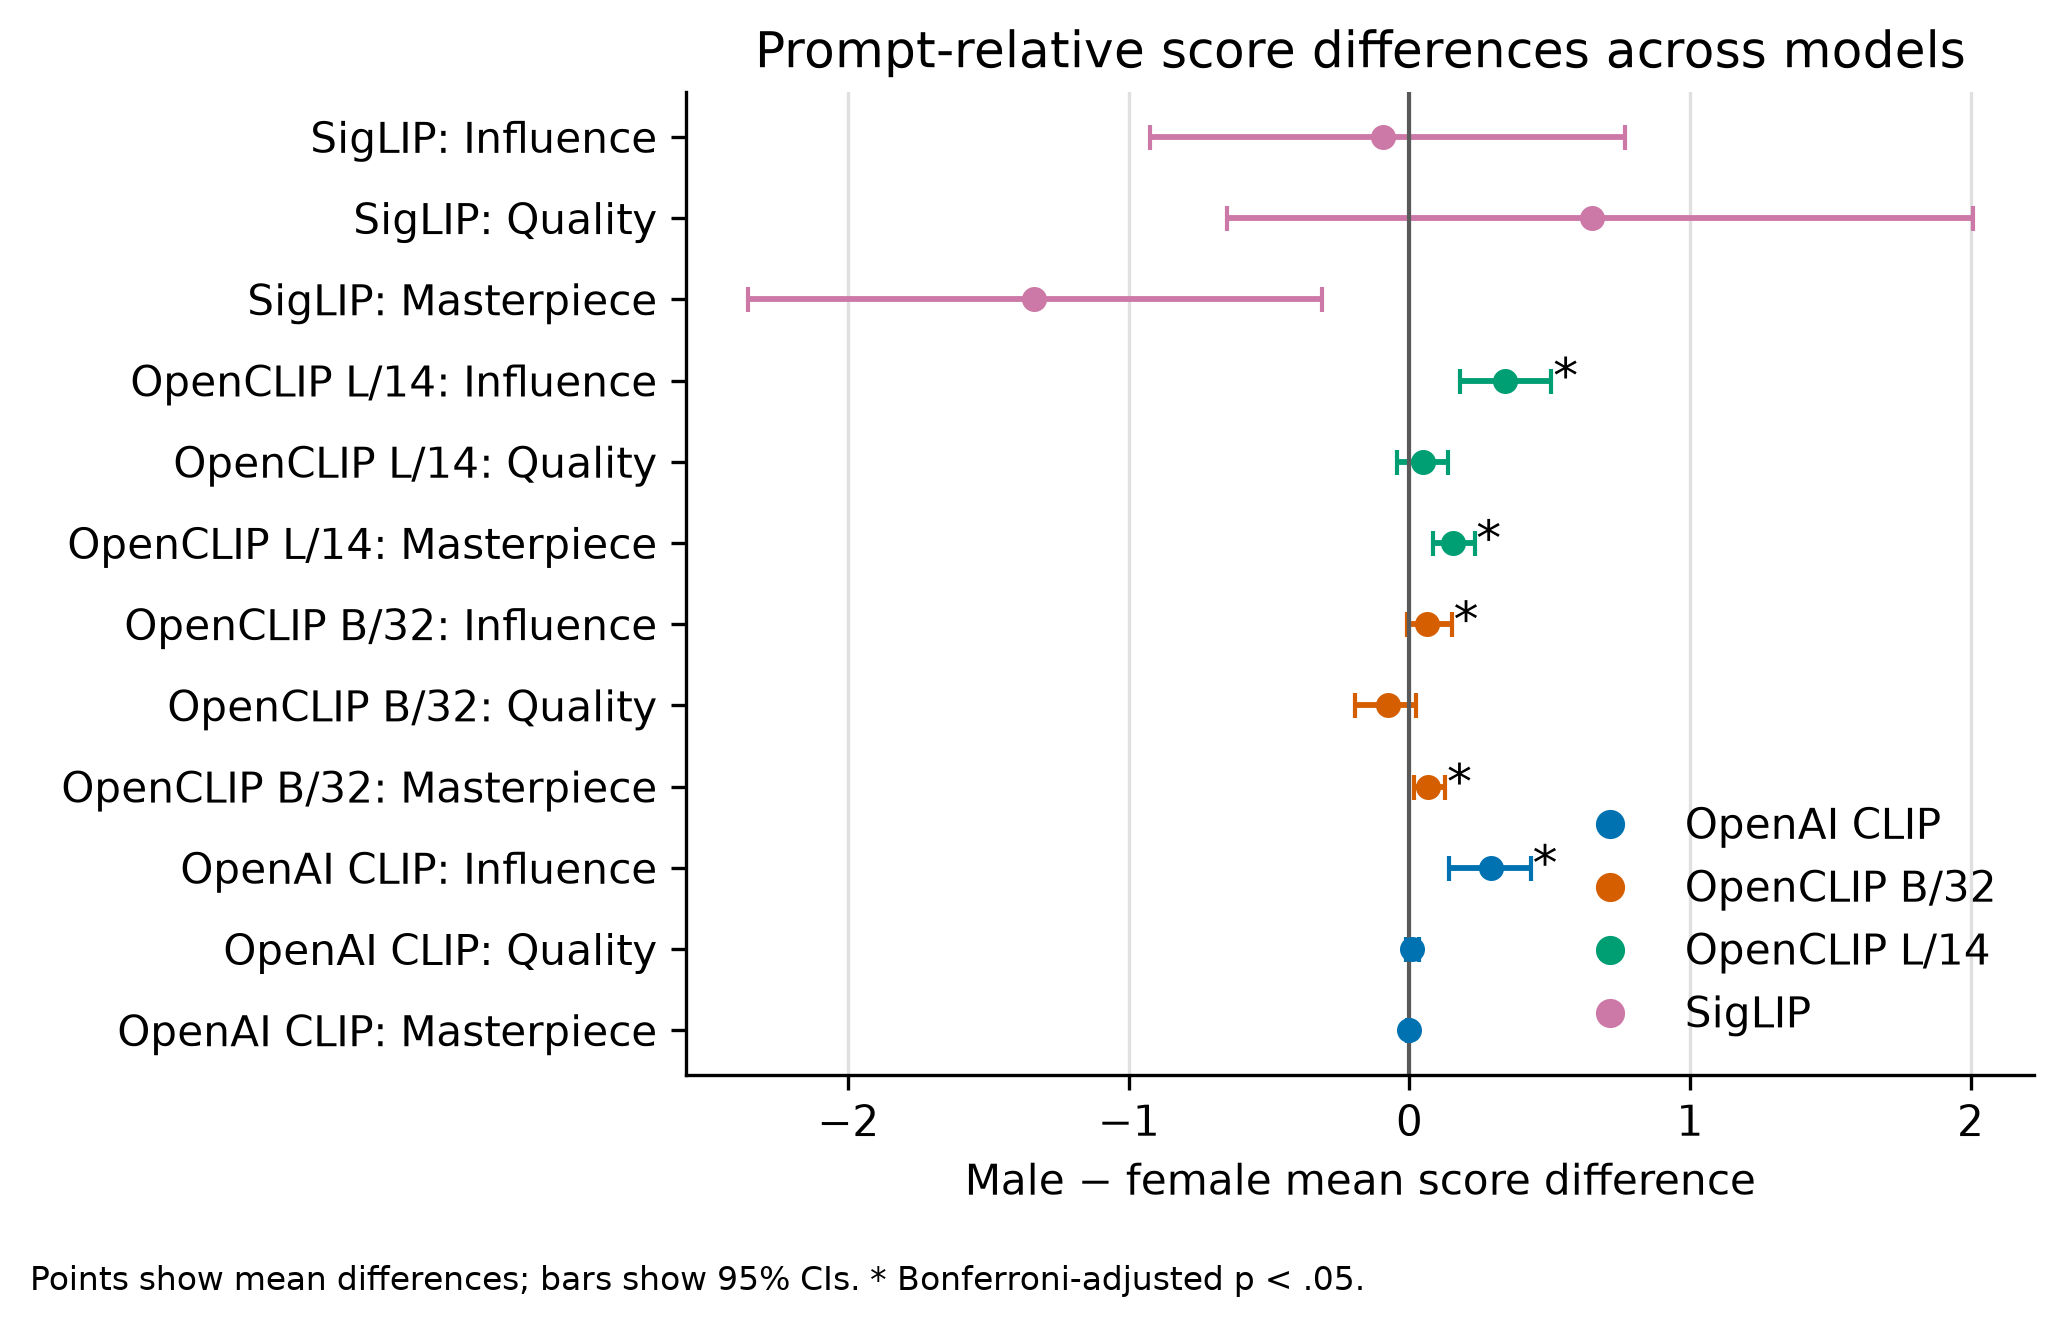
\includegraphics[width=\columnwidth]{manuscript_figures/figure_1_prompt_contrasts.png}
    \caption{Prompt-relative score differences across four vision-language models. Points show male-minus-female mean differences for the three evaluative prompt contrasts; error bars show bootstrap 95\% confidence intervals. Asterisks mark within-model Bonferroni-adjusted $p < .05$. Scores remain on native model-specific scales, so horizontal distances should be interpreted within model rather than across model families.}
    \label{fig:prompt_contrasts}
\end{figure}

\begin{figure}[htbp]
    \centering
    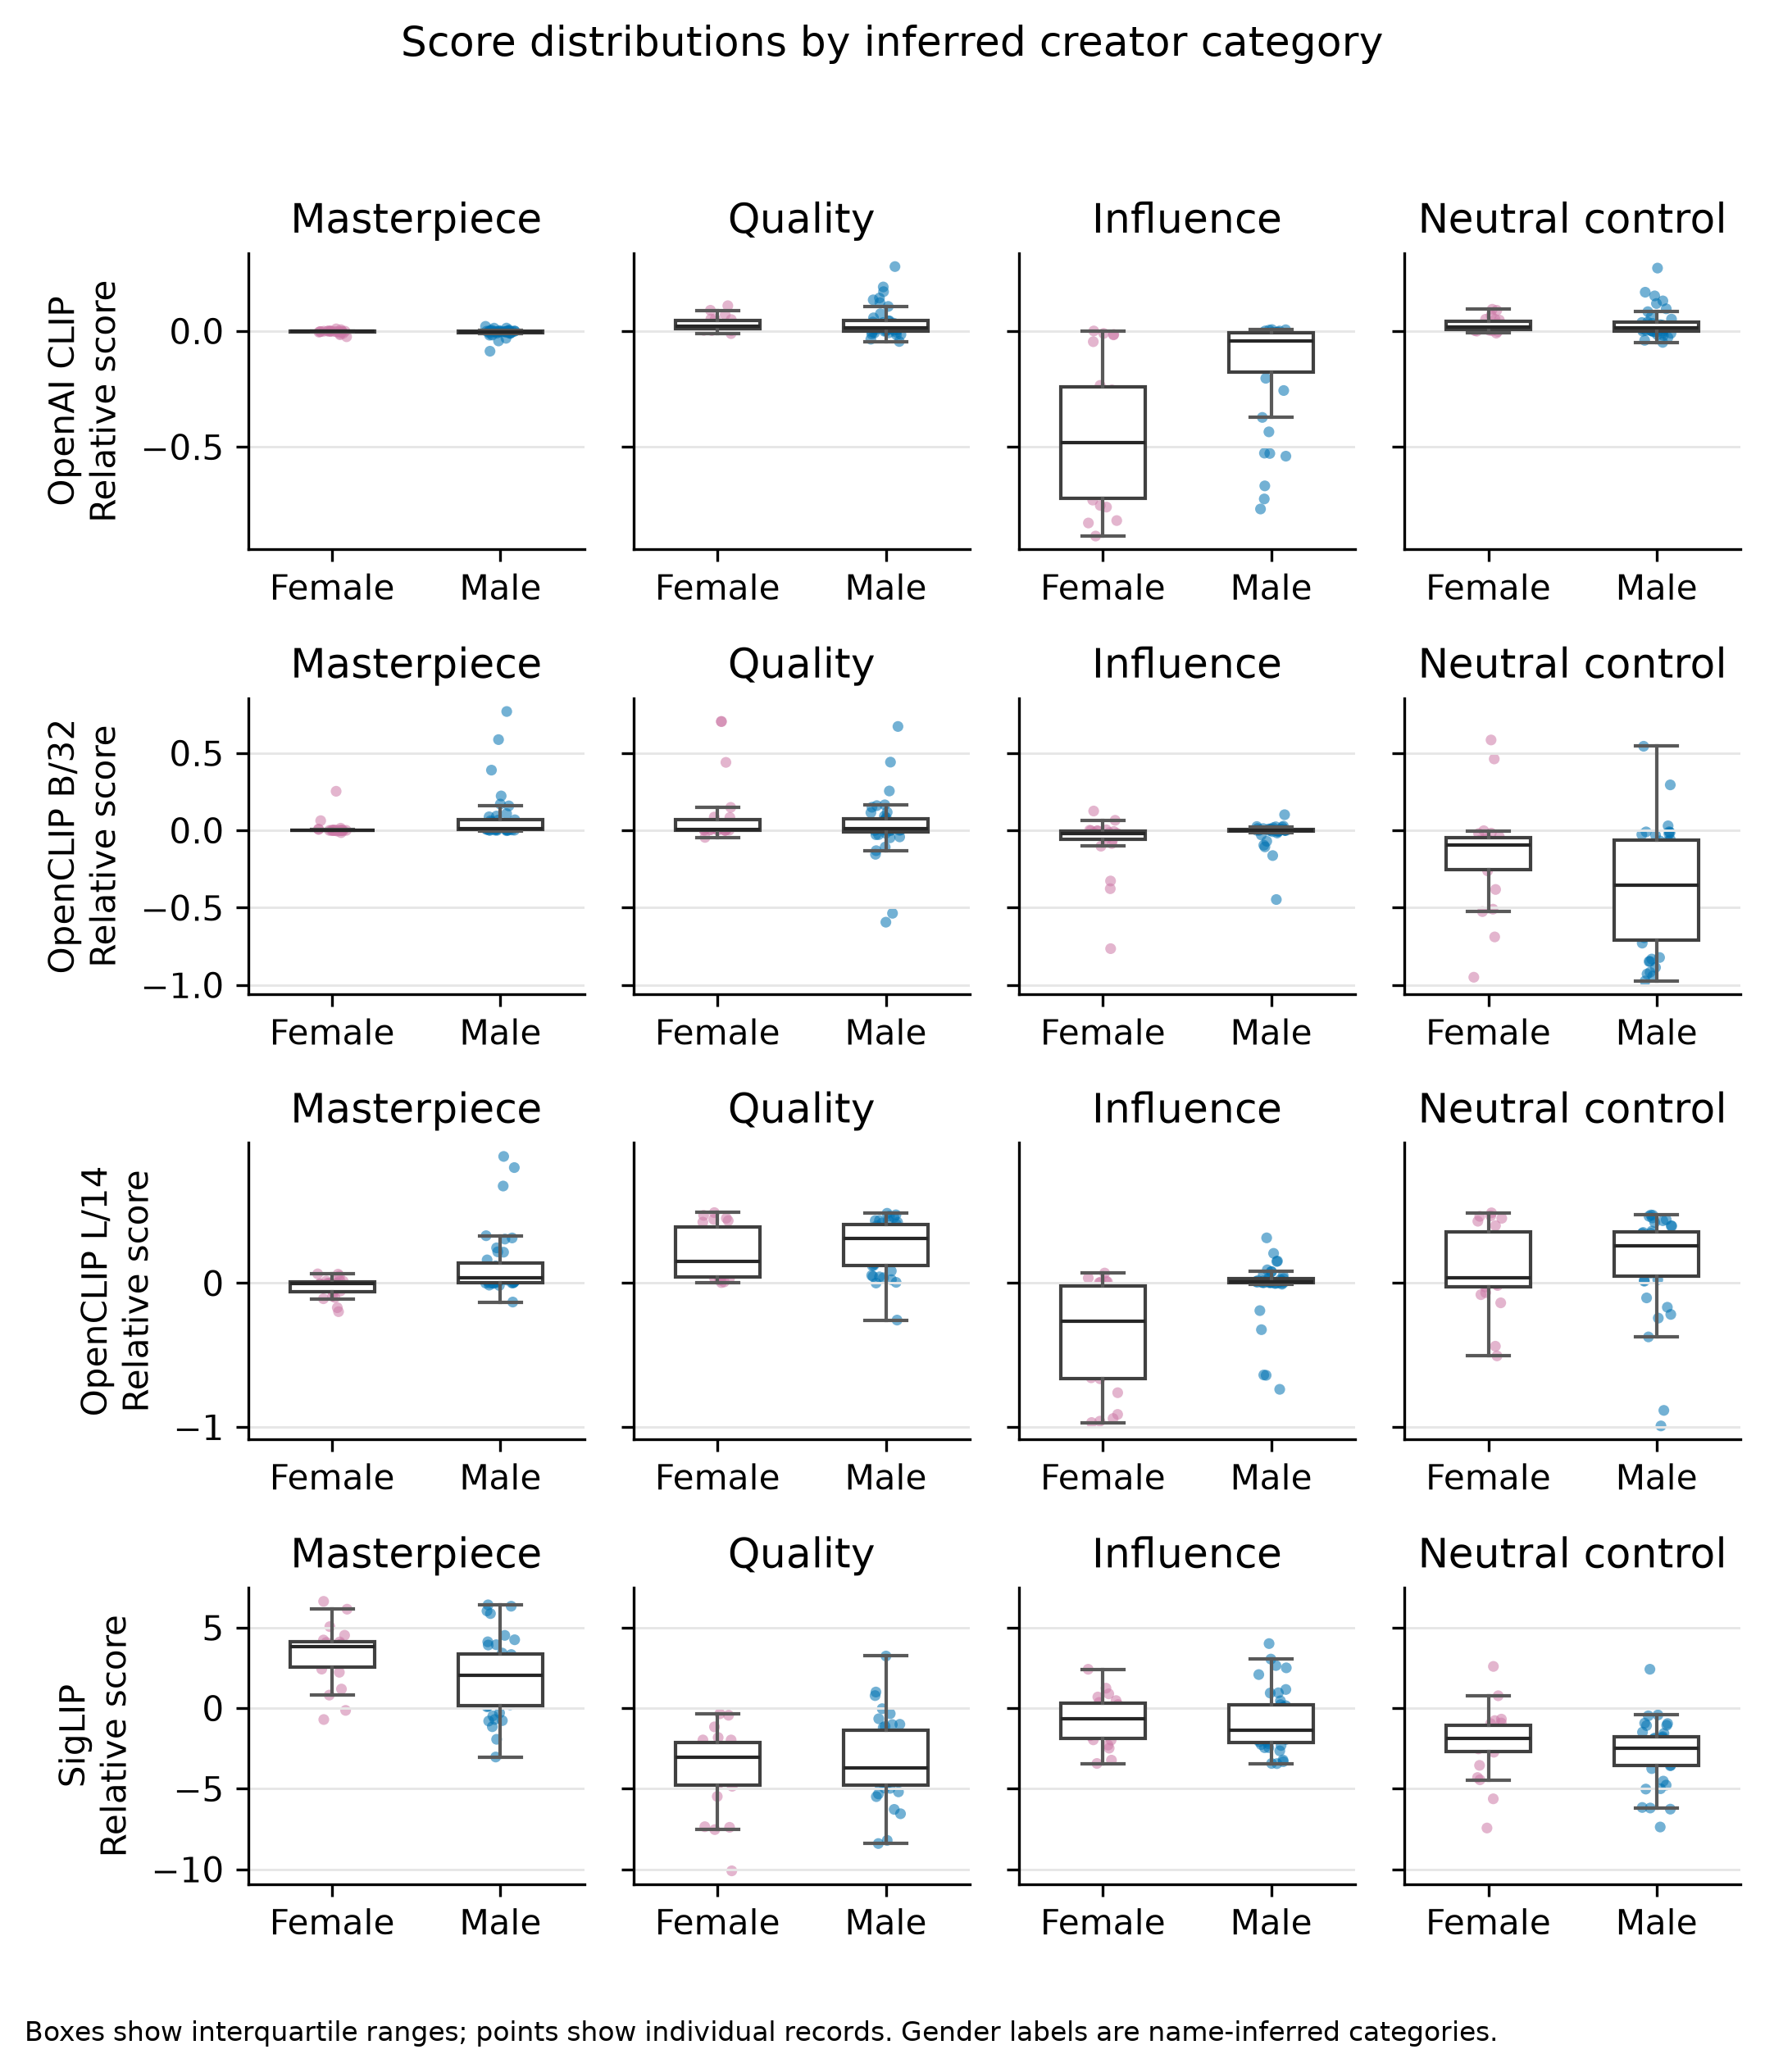
\includegraphics[width=\columnwidth]{manuscript_figures/figure_S1_score_distributions.png}
    \caption{Raw prompt-relative score distributions for male-inferred and female-inferred records. Points show individual objects and boxes show interquartile ranges. Rows separate model instances and columns separate prompt contrasts, including the framing control. Creator categories are metadata-derived analytic labels, not measures of personal gender identity.}
    \label{fig:score_distributions}
\end{figure}

\subsection{Reference diagnostics and department sensitivity}

Permutation results provide non-confirmatory reference diagnostics for prompt-specific differences. The leave-one-department-out files provide a composition check within this query-defined cohort. Because the named sample is small, department omissions can create wide intervals or unstable estimates. We use this analysis to describe cohort sensitivity, not to claim that department adjustment solves archival selection.

Permutation tests preserve observed group sizes while breaking the association between labels and scores. A small permutation $p$-value means that the observed difference is unusual under that exchangeability reference distribution. It does not mean labels are exchangeable in the archive, that data are free of confounding, or that the model has a causal gender preference. Because exchangeability is not established, these $p$-values are reference diagnostics rather than confirmatory evidence. The test is one component of the evidence, alongside effect direction, uncertainty, prompt behavior, and department sensitivity.

The department analysis has the same conditional scope. Removing a department can show that a result is concentrated in one institutional domain, but it cannot reconstruct objects absent from the collection or correct creator labels. Same-sign results across omissions indicate consistency within this query-defined cohort; they do not establish robustness beyond it. Opposite signs or wide intervals would indicate collection-composition dependence.

Table~\ref{tab:department} gives the complete leave-one-department-out results. OpenAI CLIP remains positive across all omissions, while OpenCLIP L/14 remains positive except for one imprecise omission. OpenCLIP B/32 remains negative, and SigLIP remains negative with wide intervals. These patterns support directional stability within this query-defined cohort, not universal robustness.

Department-omission results are reported in Appendix~\ref{app:supp} as exploratory composition diagnostics. They do not establish robustness beyond this query-defined cohort.

\subsection{Cross-model instability}

Cross-model diagnostics are computed only after within-model normalization. The previous raw-scale average would have mixed probability differences with SigLIP logits and is not used here. The saved object-level diagnostics report cross-model and prompt dispersion after standardization. These diagnostics identify objects for qualitative review; they are not interpreted as confirmed cases of bias, and their values are not treated as a common measurement scale.

Cross-model disagreement is not treated as noise to average away. Different pretrained models use different training mixtures, objectives, tokenizers, and implementation choices, so disagreement can reveal sensitivity in the measurement instrument itself \cite{radford2021learning, cherti2023reproducible, zhai2023sigmoid}. Object-level instability can also reflect ambiguous composition, image quality, or prompt semantics. The diagnostics identify cases for manual review; they do not turn model output into an objective annotation.

The v6 novelty-risk summary quantifies this instability across the full image-complete cohort. Across 445 objects and four models, mean cross-model standard deviation is $0.8703$, mean within-object prompt standard deviation is $1.9715$, and mean composite risk score is $3.1023$. Department-level risk is highest for Arms and Armor ($3.6304$), followed by Asian Art ($3.2319$) and The Michael C. Rockefeller Wing ($3.2239$). These values are prioritization diagnostics, not estimates of bias: they combine standardized model disagreement, prompt dispersion, and rank disagreement, and should guide qualitative review rather than label objects as erroneous or unfair.

\section{Discussion}
\label{sec:discussion}

\subsection{What the results support}

The study's contribution is a measurement protocol that keeps model, prompt, and archival selection together. In this case, some VLMs assign higher value-language scores to male-inferred works, while others do not. The result does not show universal undervaluation of women artists or validate the protocol beyond this archive \cite{wang2022revisiting, wolfe2022evidence, hall2023auditing}.

Prompt-specific results show positive influence differences for OpenAI CLIP and OpenCLIP L/14, with additional model-dependent differences for masterpiece and quality prompts. These are conditional descriptive associations under inferred metadata categories. They are not evidence that either model represents women artists negatively in every context, and the permutation values are not globally adjusted across all model-prompt analyses.

OpenCLIP B/32 and SigLIP do not reproduce the aggregate pattern, and SigLIP has the opposite direction. This disagreement rules out a universal VLM tendency and makes model choice part of the measurement procedure.

\subsection{Prompt wording as measurement choice}

Museum AI evaluations should report model and prompt dependence directly. A single prompt can produce a clear group comparison while hiding measurement instability. Multiple models help only when their score scales remain separate. The prompts ``influential,'' ``masterpiece,'' and ``quality'' are related but not interchangeable.

Prompt effects also complicate the phrase ``artistic value.'' Influence refers to historical or cultural reach, masterpiece invokes status and canon formation, and quality leaves its reference standard open. These prompts may activate different associations in the image-text model. A difference under one phrase therefore cannot be generalized to all judgments that a reader might call value. The neutral control helps identify framing sensitivity, but it is not a validated neutral baseline and cannot establish that the value prompts measure one underlying construct.

Prompt sets should be specified before subgroup inspection, justified against the target construct, and reported in full. Prompt sensitivity is a finding, not noise to average away; evaluation conditions and limitations belong beside headline metrics \cite{mitchell2019model}.

\subsection{Archival selection and causal restraint}

The archive shapes the result before model inference begins. Most objects lack a resolved creator category, and the named comparison contains only 61 works. The analysis consequently describes a selected image-complete named-attribution cohort. It does not measure the gender composition of artistic production, the museum's full collection, or human judgments of artistic quality.

The 384 unresolved records are evidence about what the catalog makes difficult to classify. Attribution practices, collective authorship, record loss, and digitization can affect entry into the named comparison. Treating them as missing completely at random would be unjustified, so the named comparison is reported as conditional on archival visibility.

Leave-one-department-out analysis can show whether an association is concentrated in one institutional domain. It cannot restore absent objects or make inferred labels equivalent to verified identities. A result that survives department omissions is more stable within this collection, not necessarily portable to another museum. This follows the broader archival point that categories and retrieval systems participate in what becomes available for analysis \cite{bowker2000sorting, caswell2016archival}.

\subsection{Implications for museum AI audits}

For cultural-heritage institutions, the implication is methodological. A model score should not rank artistic worth, replace curatorial judgment, or guide acquisition and deaccession. Museum applications must distinguish image associations from institutional judgments \cite{fiorucci2020machine, srinivasan2021arts}.

An audit record should include source collection, image-selection rule, unresolved-label count, exact prompts, model scales, correction family, permutation scheme, and sensitivity outputs. Opposite results under another model, prompt, or collection should be treated as evidence about transportability and instrument dependence.

The protocol therefore requires model-specific results, within-model normalization, explicit selection accounting, and unknown-category reporting. It cannot remove bias from archives or models, but it prevents a fragile comparison from being presented as a general measure of cultural value.

\section{Limitations and ethics}
\label{sec:limitations}

\subsection{Data and label limitations}
The 39 versus 22 comparison is vulnerable to influential objects, departments, and shared creators. Leave-one-object-out ranges describe sensitivity within this query-defined cohort; intervals do not represent uncertainty over artists or the museum population. Creator-clustered analyses remain unavailable because attribution identifiers are incomplete.

The comparison sample is small and unbalanced: 39 male-inferred and 22 female-inferred records, with 384 unresolved records. The binary contrast therefore uses 13.7\% of the image-complete cohort and has limited power for modest effects or population-level estimates. Metadata-inferred creator categories come from museum fields and name lookup, not verified identities; name dictionaries have uneven geographic and historical coverage, and catalog fields may encode institutional assumptions \cite{keyes2018misgendering, buolamwini2018gender}.

One institution cannot establish external validity. The Metropolitan Museum of Art has its own collecting history, departments, catalog conventions, digitization priorities, and image policies. A different museum, region, period, or image corpus could produce different results. The image-complete cohort is also not a random sample of museum records, and the named subset is not a random sample of artists. The findings should therefore be generalized only to similar audit conditions unless replicated elsewhere.

\subsection{Measurement and statistical limitations}
The permutation reference assumes exchangeability of the inferred labels conditional on the observed cohort. That assumption is a useful reference for the score contrast, but it is not a model of how archival labels were produced. The current results should not be read as correcting department, medium, period, image-quality, or selection imbalance. Restricted permutations or matched analyses by collection strata would provide a stronger robustness check.

Prompts lack independent human validation and differ in semantic scope. Weak or mixed correlations do not support treating the aggregate as reliable. A larger difference may reflect wording, image composition, or training associations rather than artwork evaluation.

No human baseline was collected, so agreement with expert or public judgments cannot be assessed. Results concern specified text-image pairs, not human artistic-value judgments. Diverse human panels are needed for construct validation.

Model scores may reflect image composition, medium, period, framing, resolution, color, and catalog practice. The present metadata variables cannot capture all of these factors. Covariate adjustment cannot identify causal effects in this observational archive, and department adjustment may remove historical structure rather than correct it. Regression or leave-one-department-out stability would still be conditional evidence.

The object is the unit used in the current tests, but objects may not be independent in a historical collection. Multiple works can share a creator, workshop, department, image convention, or cataloging practice. Creator-clustered or cluster-level permutation analyses are not available because the metadata do not provide a consistently resolved creator identifier for the full cohort. The reported uncertainty should therefore be read as object-level conditional uncertainty, not as a fully cluster-robust estimate over artists or institutions. The creator-display-string counts reported in Methods show why object-level results should not be generalized to creators. Future analyses should repeat the comparison with creator-level clustering after expert-reviewed attribution data are available.

The stated Bonferroni family covers four value contrasts within each model, not every prompt, subgroup, diagnostic, or future analysis. Bootstrap intervals likewise describe the named cohort, not missing objects, labels, images, or the museum population.

SigLIP logits and CLIP probabilities require separate interpretation. Raw magnitudes cannot be ranked across families; standardization does not create semantic equivalence. Report cross-model agreement by direction, rank, or standardized behavior, not pooled scores.

\subsection{Ethical boundaries and responsible use}

The study was carried out by means of public catalog metadata and artwork images obtained through the Metropolitan Museum of Art Open Access API. Although the API is available to the public, this does not mean that unrestricted commercial rights are granted, as such rights are still governed by the terms applicable to each individual record. The audit focuses solely on the artwork records and does not classify any of the people who are depicted in the images, choosing instead to keep objects that are either unknown or unattributed rather than forcing them into either-or categories.
The empirical results should not be employed for ranking artists, for assessing artistic merit, for automating curatorial procedures, or for guiding policies on collection acquisitions. A lower prompt-relative model score does not mean that the artistic quality is inferior, and a statistically identifiable difference in scores does not prove the presence of intentional developer bias. Rather, these metrics offer diagnostic information about how multimodal models handle cultural artifacts under given prompt and metadata conditions. Before making any institutional decisions, responsible use involves combining the audit diagnostics with qualitative historical analysis \cite{jobin2019global, stahl2021responsible}.
The fact that some attributions have not been resolved, that there are missing image records, and that there are disagreements between different models represents important analytical findings. Further research should extend this procedure to include collections from various institutions, use attributions that have been curated by experts, and at the same time assess the responses to the prompts against panels consisting of different human experts.


\section{Conclusion}
\label{sec:conclusion}

Vision-language models do not offer a single, overall assessment of artistic value. To address this, we developed an archive-conditioned audit procedure which incorporates model selection, the way prompts are phrased, and the catalog metadata into one evaluation framework. In our test group drawn from the Metropolitan Museum of Art, some models obtained higher value-language scores when the prompts suggested male-inferred creators, while with other models and prompts the results were either inconsistent or even opposite. The differences in these scores are due to the text-image associations that occur under specific prompts and metadata heuristics, not because of general model biases or any absolute measure of artistic quality.
Our results give a clear recommendation with regard to methodology: when evaluating multimodal AI in cultural heritage contexts it is necessary to record the archival filtering steps, try out various prompt versions, carry out different label sensitivity arrangements, examine the collection strata, and keep the raw score scales separate for each model family. In the case of auditing complex cultural areas, the disagreement between models serves as meaningful evidence of evaluation uncertainty rather than as statistical noise which should be smoothed out.

\appendix
\section{Supplementary sensitivity results}
\label{app:supp}

These tables are exploratory composition diagnostics. Differences are male-minus-female contrasts between metadata-inferred creator categories. Permutation values are reference diagnostics only because exchangeability is not established. They do not measure artistic quality, creator identity, or causal model preference. Full regression outputs, where retained, belong in the supplementary package rather than the main text.

\begin{table}[htbp]
\centering
\caption{Aggregate prompt index by model. Secondary descriptive summary.}
\label{tab:mainresults}
\scriptsize
\begin{tabular}{lrrrrr}
\toprule
Model & Male mean & Female mean & Difference & Reference $p$ & Bonferroni $p$ \\
\midrule
OpenAI CLIP & $-0.0235$ & $-0.0989$ & $0.0757$ & $0.0005$ & $0.0027$ \\
OpenCLIP B/32 & $-0.0732$ & $-0.0307$ & $-0.0424$ & $0.2168$ & $0.5096$ \\
OpenCLIP L/14 & $0.1248$ & $-0.0234$ & $0.1487$ & $0.0016$ & $0.0153$ \\
SigLIP & $-1.2096$ & $-0.8644$ & $-0.3457$ & $0.1995$ & $0.5403$ \\
\bottomrule
\end{tabular}
\end{table}

\begin{table*}[htbp]
\centering
\caption{Leave-one-department-out aggregate sensitivity. Intervals are bootstrap 95\% intervals. Reference values are not confirmatory $p$-values.}
\label{tab:department}
\scriptsize
\begin{tabular}{llrr}
\toprule
Model & Omitted department & Difference & 95\% interval \\
\midrule
OpenAI CLIP & Arms and Armor & 0.0767 & [0.0368, 0.1160] \\
 & Asian Art & 0.0756 & [0.0377, 0.1133] \\
 & Medieval Art & 0.0777 & [0.0383, 0.1161] \\
 & Musical Instruments & 0.0782 & [0.0385, 0.1168] \\
 & Robert Lehman Collection & 0.0634 & [0.0190, 0.1075] \\
 & The American Wing & 0.0831 & [0.0367, 0.1271] \\
 & Michael C. Rockefeller Wing & 0.0448 & [-0.0044, 0.0970] \\
\midrule
OpenCLIP B/32 & Arms and Armor & -0.0387 & [-0.1073, 0.0248] \\
 & Asian Art & -0.0441 & [-0.1083, 0.0190] \\
 & Medieval Art & -0.0431 & [-0.1110, 0.0202] \\
 & Musical Instruments & -0.0418 & [-0.1088, 0.0216] \\
 & Robert Lehman Collection & -0.0320 & [-0.1195, 0.0534] \\
 & The American Wing & -0.0200 & [-0.0679, 0.0327] \\
 & Michael C. Rockefeller Wing & -0.0673 & [-0.1733, 0.0268] \\
\midrule
OpenCLIP L/14 & Arms and Armor & 0.1478 & [0.0583, 0.2330] \\
 & Asian Art & 0.1508 & [0.0619, 0.2353] \\
 & Medieval Art & 0.1442 & [0.0561, 0.2266] \\
 & Musical Instruments & 0.1559 & [0.0690, 0.2378] \\
 & Robert Lehman Collection & 0.1286 & [0.0292, 0.2228] \\
 & The American Wing & 0.1699 & [0.0554, 0.2793] \\
 & Michael C. Rockefeller Wing & 0.0778 & [-0.0281, 0.1845] \\
\midrule
SigLIP & Arms and Armor & -0.3187 & [-0.8207, 0.2134] \\
 & Asian Art & -0.3854 & [-0.8762, 0.1240] \\
 & Medieval Art & -0.3127 & [-0.8130, 0.2098] \\
 & Musical Instruments & -0.3648 & [-0.8672, 0.1586] \\
 & Robert Lehman Collection & -0.7172 & [-1.3911, -0.0069] \\
 & The American Wing & -0.0722 & [-0.6209, 0.4698] \\
 & Michael C. Rockefeller Wing & -0.4179 & [-1.0732, 0.2669] \\
\bottomrule
\end{tabular}
\end{table*}

\section*{Declarations}
\begin{itemize}
\item \textbf{Funding}: This research received no specific grant from any funding agency.
\item \textbf{Conflict of interest}: The authors declare no competing interests.
\item \textbf{Ethics approval}: The study uses publicly available museum metadata and images and involves no human participants.
\item \textbf{Data availability}: Museum metadata and image records were obtained through the Metropolitan Museum of Art Open Access API. Availability and reuse of individual images remain subject to the museum's record-level terms.
\item \textbf{Code availability}: Code, manifests, prompts, requirements, and analysis outputs are included in the public repository at \url{https://github.com/manpreet28111995/disentangling-archival-bias}. The authors will archive the submitted revision with a release identifier and commit hash.
\item \textbf{Author contributions}: The authors contributed to study design, analysis, interpretation, and manuscript preparation. All authors approved the submitted version.
\item \textbf{Use of AI-assisted tools}: AI-assisted tools were used during manuscript editing and software review. The authors retained responsibility for study design, code, statistical analysis, interpretation, citations, and final text.
\end{itemize}

\bibliography{Bibliography}
\end{document}
